\chapter{Allgemein}

%(Separate) Dokumentation notwendig
%formlos 5-10 Seiten
%Thema, Motivation, ggf. Bedienung des Programms
%Begründung der wichtigen Design-Entscheidungen bei der Umsetzung

% Allg. Text bezueglich Juce und PLuginFormaten

Um Musik am Computer zu produzieren werden verschiedene Synthesizer und Effekte benutzt. Diese sind oftmals in C++ programmiert. Wichtig ist hierbei die Unterstützung von dem Musikprogrammen (Ableton Live) und das Wissen über verschiedene Plugin Formate.

\section{JUCE}

Juce ist ein C++ Framework zur Erstellung von Desktop und mobilen Anwendungen. Das Framework ist Open-Source und kann von dem GitHub-Repository heruntergeladen werden. Dort sind verschiedene Wrapper-Klassen enthalten die es ermöglichen, Audio Anwendungen zu erstellen \cite{JUCE}. 

Die Besonderheit von Juce bildet das Tool Projucer. Dieses Tool ist eine IDE zum Erstellen und Verwalten von Juce Projekten. Mit ein paar Klicken erstellt dieses Tool für jede gewünschte Plattform ein Projekt. Zum Beispiel kann eingestellt werden, dass ein Visual Studio 2017 und ein XCode Projekt erstellt werden kann. Bei Projekte verwenden den selben Sourcecode. In den Projekten selber werden, je nach Auswahl, weitere Projekte erzeugt abhängig davon, welche Plugin Formate erstellt werden sollen.

\begin{figure}
	\centering
	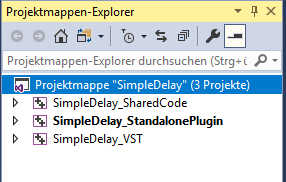
\includegraphics[width=0.7\linewidth]{images/projektmappe}
	\caption{VS '17 Projektmappen-Explorer. Erstellen des Projekts erzeugt hier ein .exe und ein VST2 Plugin (.dll)}
	\label{fig:projektmappe}
\end{figure}

Der Projucer erzeugt ein kleines Programmcodeskelett mit nützlichen Standardfunktionen. Dies vereinfacht den Einstieg, so dass nicht viel Zeit mit der Einarbeitung von irgendwelchen SDKs verschwendet wird.

\section{Plugins}

%Formate
In der heutigen Musikproduktion werden verschiedene Formatstandards für Plugins eingesetzt. Die Wahl für einen gewissen Standard ist abhängig von dem gewählten Betriebssystem sowie welche digitale Audioworkstation (DAW) verwendet wird. Um festzustellen, welche Formate von der jeweiligen DAW unterstützt wird, sollte die Herstellerwebseite bezogen werden. Die Formate unterscheiden sich in ihrer Funktion nicht großartig. Dazu eine kleine Liste von bekannten Formaten und unterstützenden DAWs \cite{PF}:

\begin{itemize}
	\item VST (Virtual Studio Technology): Ableton Live, Fl Studio, Cubase, Reason, Reaper
	\item AU (Audio Unit)[Nur Mac]: Ableton Live, Logic Pro, Studio One 
	\item RTSA (Real Time AudioSuit): Pro Tools
	\item AAX (Avid Audio eXtension): Pro Tools
\end{itemize}

Steinberg stellt zur Erstellung von VSTs ein SDK bereit. Im Moment beginnt bei Steinberg eine Umstellung von dem VST2 Standard auf den VST3 Standard. In der aktuell verfügbaren SDK gibt es keine Unterstützung mehr für die Erstellung von VST2 Plugins. Manche Hersteller haben sich noch nicht angepasst wie zum Beispiel Ableton, diese akzeptieren bislang noch keine VST3 Plugins. Ältere Versionen von Juce haben noch einen VST2 Support zum Erstellen von Plugins. Die aktuelle Version kann jedoch nur noch den neusten VST Standard erzeugen.
Da zum Testen stand nur Ableton zu Verfügung, weshalb das Plugin mit einer älteren Version von Juce erstellt werden musste. Das Plugin selber ist eine .dll-Datei, welche sich im VST-Plugin Ordner der DAW befinden muss. Wichtig ist, dass das Plugin und die DAW die selbe Bit-Architektur haben (32/64).